\subsection{KNN}
Analisis de KNN

\subsubsection{Cantidad de vecinos}
Mover el k y presentar un analisis

\subsubsection{Mejoras en kNN}
Cortar el dataset en x valor y comparar para ver si mejora

\subsection{PCA}
Analisis de PCA
Ahora vamos a analizar el algoritmo del PCA.
Vamos a probar el algoritmo para distintas medidas de k y $\alpha$, que van a ser:
k: cantidad de vecinos a considerar en el algoritmo kNN.
$\alpha$: a la cantidad de componentes principales a tomar.

Vamos a probar el algoritmo para los siguientes valores:
k:
$\alpha$: 

Lo que vamos a probar es fijando un valor de lamda, para que cantidad de vecinos vamos a tener la mayor cantidad de aciertos, y asi, maximizar la cantidad de aciertos.
Nosotros despues de aplicar el algoritmo pca, aplicamos el knn y armamos una cola de prioridad para los resultados de aplicar el algoritmo knn. Lo que se hace es agarrar dos imagenes, restarlas y aplicarle la norma2 para saber en cuanto difieren una imagen y la otra. El la cola de prioridad, estan adelante los valores mas chicos, o sea, las imagenes del test que mas cerca de coincidir estan con respecto a la imagen de la base de datos.
Por lo tanto, si elegimos mas cantidad de vecinos, lo que nos puede pasar son dos cosas:
1) Que sea beneficioso ya que a mayor cantidad de pruebas vamos a tener mas aciertos
2) Que sea malicioso ya que a mayor cantidad de pruebas vamos a obtener peores datos, o sea, vamos a mirar las imagenes que menos coiciden con la imagen de prueba de la base de datos.

La conclusion que llegamos es que a mayor cantidad de vecinos, el algoritmo empieza a funcionar peor, ya que estamos mirando los vecinos que menos coinciden con la base de datos, porque la cola de prioridad los ordena segun menos diferencias haya entre la foto obtenida y las fotos de la base de datos. 
Por lo tanto, cuanto mas vecinos exploro, menos cantidad de aciertos obtengo. Eso lo puedo ver a traves de las siguientes mediciones realizadas para distintos k vecinos y fijando un valor de lamda.

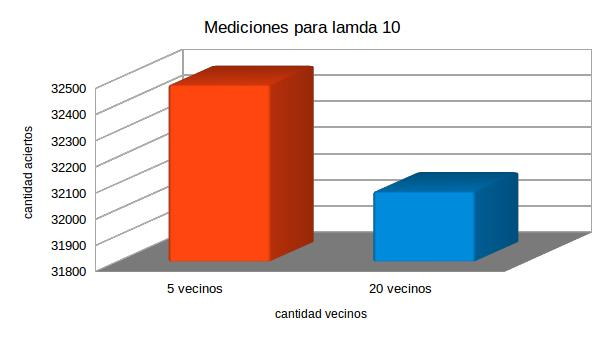
\includegraphics[scale=0.75]{lamda10.jpg}\\
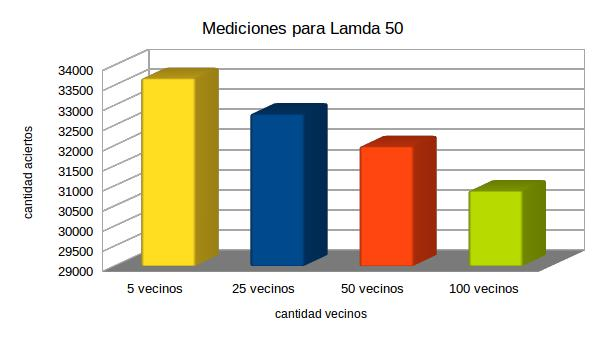
\includegraphics[scale=0.75]{lamda50.jpg}\\
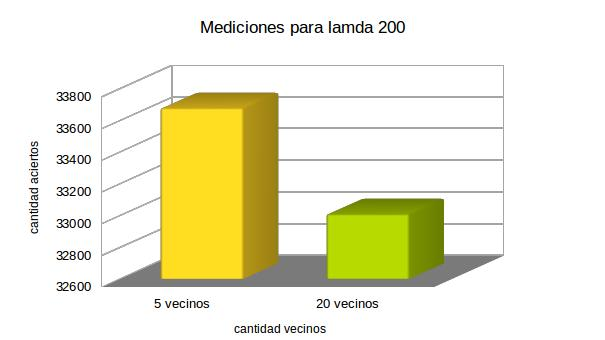
\includegraphics[scale=0.75]{lamda200.jpg}\\
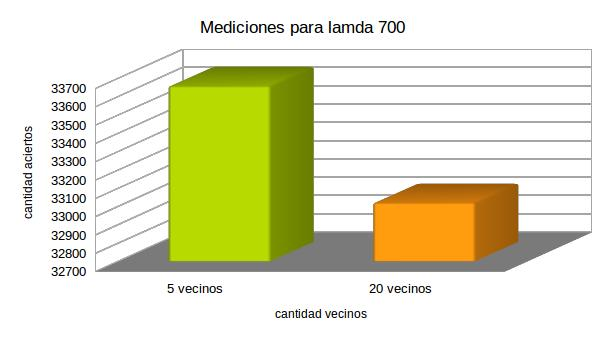
\includegraphics[scale=0.75]{lamda700.jpg}\\


Otra conclusion que sacamos es que para k=5 vecinos es la mejor cantidad de vecinos para obtener la mayor cantidad de aciertos. 
Ahora, ¿No seria mejor agarrar solo el primero de la cola de prioridad, o sea, k=1? 
Lo que podria pasar es que el unico vecino que agarremos, sea el mejor pero no alcance para saber cual es el digito de la imagen, ya que si no se acierta con el unico vecino que elegi, me podria fallar el digito del resultado y eso reduciria muchisimo la cantidad de aciertos.

\subsubsection{Lambda inicial}

\subsubsection{Algo mas que no me acuerde}
